\section{MPPDC: Model Prediction-based Perceptual Deformation Control Strategy}\label{sec:propose}

\begin{figure}
    \centering
    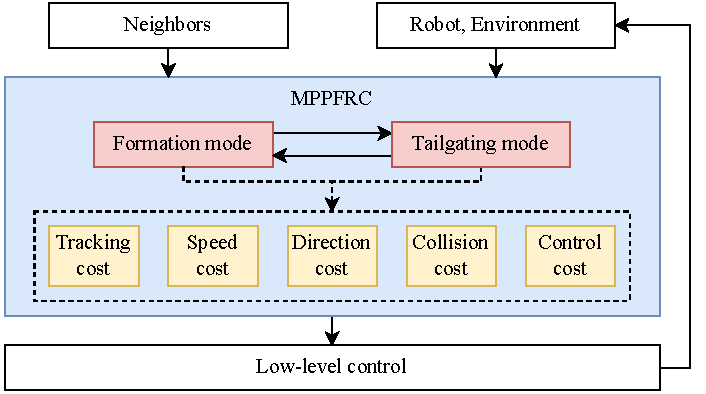
\includegraphics[width=0.7\textwidth]{paper3/images/diagram.pdf}
    \caption{The diagram of the proposed method implemented for each robot. The point cloud data of the environment observed from local sensors and the information from the neighbors are collected as inputs to the proposed approach. Our predictive control strategy, which includes two primary modes: \textit{``Formation''} and \textit{``Tailgating''}, is formulated by the weighted-sum of five cost functions to address the requirements \textit{(O1-O4)}. The optimal solver is constructed to generate the control signal for the low-level controller.}
    \label{fig:diagram}
\end{figure}

In this work, the formation of robots has the mission to pass through a narrow environment. During the movement, the formation is required to \textit{(O1)} maintain their shape; \textit{(O2)} move along to the predefined direction $u_\text{ref}\in\mathbb{R}^{3}$, where $\left\Vert u_\text{ref}\right\Vert=1$, which can be determined by information collected from surrounding environments~\cite{9565893,Matveev2020}, with \textit{(O3)} the desired speed $\bar{v}_\text{ref}\in\mathbb{R}$; and \textit{(O4)} ensuring no collision with other neighbors or obstacles in the environment.

The proposed deformation control strategy is illustrated in Fig.~\ref{fig:diagram}, which contains two modes, \textit{``Formation''} and \textit{``Tailgating''}. Based on the point cloud data obtained from a local sensor equipped on each robot, the formation can be switched from \textit{``Formation''} to \textit{``Tailgating''} mode if the width of the environment is too narrow to maintain the whole formation topology. In \textit{``Formation''} mode, the formation can maintain its original shape, and in \textit{``Tailgating''} mode, the formation transforms into straight line shapes with positions determined based on their orientation relative to the specified direction $u_\text{ref}$. The straight line shape is chosen in our work because it is an effective shape that can be used to go through obstacles like narrow valleys or tunnels~\cite{Fu2020}.

In the \textit{``Formation''} mode, the aim is to maintain the desired given shape. Let $\delta_{ij}\in\mathbb{R}^3,\forall j\in \mathcal{N}_i$ be the vector representing the desired position of robot $i$ with respect to neighbor $j$. Note that $\delta_{ji}=-\delta_{ij}$ must be satisfied for all pairs $\left(i,j\right)$, $j\neq i$, for consistency and feasibility of the formation. Note also that $\delta_{ii}=0$ for all $i$. This aim can be given as follows~\cite{Dong2016,6798711}:
\begin{equation}
    \lim_{k\to\infty}{\left(p_j(k)-p_i(k)+\kappa\delta_{ij}\right)}=0,\quad\forall i,j\in\{1,...,N\}, i\neq j
\end{equation}
where $\kappa\in[0,1]$ is the scaling factor representing the shrinkage of the formation. This scaling factor can be determined by the environment's width in Section~\ref{sec:obs_aware}. As a result, the desired relative position of every robot $i$ in the formation can be described as follows:
\begin{equation}
    p^*_i(k)=\dfrac{1}{N_i}\sum_{j\in\mathcal{N}_i}{\left(p_j\left(k\right)+\kappa\delta_{ij}\right)}
    \label{eqn:formation}
\end{equation}

In addition, to determine the leader robot, the inner product $\tilde{p}_{ij}$ of the difference between robot $j$ in the neighbor set $\mathcal{N}_i$ with robot $i$, $p_j-p_i$, and the desired direction, $u_\text{ref}$, is given as follows:
\begin{equation}
    \tilde{p}_{ij} = \left\langle (p_j-p_i),u_\text{ref}\right\rangle
    \label{eqn:tildep}
\end{equation}

As a result, the value of $\tilde{p}_{ij}$ is positive, proving that robot $j$ is in front of robot $i$ according to $u_\text{ref}$, and vice versa. For all robots $j$ in the neighbor set $\mathcal{N}_i$, we obtain $\mathcal{P}_i=\left\{\tilde{p}_{ij}\right\}$. The leader robot ${l_i}$ of robot $i$ is chosen as the closest robot in front of it, i.e.
\begin{equation}
     l_i=\begin{cases}
    \arg\min_{j}\left\{\tilde{p}_{ij}\in\mathcal{P}_i\vert\tilde{p}_{ij}\geq0\right\} & \exists~\tilde{p}_{ij}\geq0\\ 
    -1 & \text{otherwise}
     \end{cases}
    \label{eqn:li}
\end{equation}

The leader selection process is presented in Alg.~\ref{alg:ls}.
\begin{algorithm}
\caption{Pseudocode of leader selection}
\label{alg:ls}
\ForEach{$j\in\mathcal{N}_i$}{
    Compute inner product $\tilde{p}_{ij}$\tcc*[r]{Eq. \ref{eqn:tildep}}
    $\mathcal{P}_i\leftarrow\tilde{p}_{ij}$\;
}
Select the leader $l_i$ to follow\tcc*[r]{Eq. \ref{eqn:li}}
\Return $l_i$\;
\end{algorithm}

On the other hand, the \textit{``Tailgating''} mode allows robot~$i$ to follow robot~$j$ and keeps a distance~$\bar{d}_\text{ref}\in\mathbb{R}$ with robot~$j$, to form the straight line shape. This mode is enabled when the operation space becomes too narrow to maintain the original formation as the inter-agent collision might occur. At that time, the tailgating strategy is essential for the swarm so that each robot can move one after another through the narrow passage without collision. Assume robot~$i$ follows robot~$j$ with the desired distance~$\bar{d}_\text{ref}$. The following conditions must be satisfied:
\begin{equation}
    \lim_{k\to\infty}{\left\Vert p_j(k)-p_i(k)\right\Vert}=\bar{d}_\text{ref}
\end{equation}

In order to allow robot $i$ to follow the robot~$j$ and keep a desired distance~$d_\text{ref}$ with robot~$j$, the desired relative position of robot~$i$ can be expressed as follows:
\begin{equation}
    p_i^*(k)= p_j(k)-\bar{d}_\text{ref}u_\text{ref}
    \label{eqn:tailgating}
\end{equation}

Therefore, the requirement of shape maintenance \textit{(O1)}, i.e. formation maintenance in \textit{``Formation''} mode and following in \textit{``Tailgating''} mode, can be synchronized into a tracking objective that is represented by desired position $p_i^*$ to reduce the complexity of the optimization process. 

\subsection{The predictive control formulation}
This section describes our proposed predictive strategy. Denote $P\in\mathbb{N}^+$ as the prediction horizon, which is finite and shifts forward at every time step. Let $(\cdot)(k+l|k )$ be the predicted value of $(\cdot)(k+l )$ with the information available at time $t(k)$ and $l \in\{0,...,P\}$. Then, the condition of the robot state is written as follows:
\begin{equation}
    x_i(k|k)=x_i(k)
\end{equation}

Let $X_i(k)\in\mathbb{R}^{6P}$ be the stacked sequence of the predicted states $x_i(k+l|k)$ over the horizon $l\in\{1,...,P\}$ and $U_i(k)\in\mathbb{R}^{3P}$ the stacked sequence of the predicted control inputs $u_i(k)$ over the horizon $l\in\{0,...,P-1\}$. To resolve the formation requirements, we modeled those requirements into candidate cost functions, i.e. \textit{(O1)} tracking cost $J_{t,i}(k)$, \textit{(O2)} speed cost $J_{s,i}(k)$, \textit{(O3)} direction cost $J_{d,i}(k)$, \textit{(O4)} collision costs, including obstacle avoidance cost $J_{o,i}(k)$, and inter-agent collision cost $J_{i,i}(k)$, and an addition control cost $J_{u,i}(k)$ is a penalty term to get the minimal solution. Hence, the distributed formation control system can be modeled by the non-convex optimization problem as follows:
\begin{equation}
\begin{aligned}
    \min_{U_i(k)}&\left(J_{t,i}(k)+J_{s,i}(k)+J_{d,i}(k)+\right.\\
    &\left.J_{o,i}(k)+J_{i,i}(k)+J_{u,i}(k)\right)
\end{aligned}
    \label{eqn:J}
\end{equation}
subject to:
\begin{equation}
    \begin{aligned}
        &x_i(k+l+1|k)=Ax_i(k+l|k)+Bu_i(k+l|k),\\
        &x_i(k|k)=x(k),\\
        &v_\text{min}\leq v_i(k+l|k)\leq v_\text{max},\\
        &u_\text{min}\leq u_i(k+l|k)\leq u_\text{max},\\
    \end{aligned}
    \label{eqn:constraints}
\end{equation}
with $l\in\{1,...,P\}$, and $i\in\mathcal{N}$.

\subsubsection{Tracking term}\label{sec:tracking_term}
The tracking term for robot $i$ at time $t(k)$ aims to optimize the following square error between the desired position~$p_i^*$ and the  predicted position~$p_i$, thus, the robot~$i$ is encouraged to closely track its desired position, leading to more accurate and reliable path following. This term is defined as follows:
\begin{equation}
    J_{t,i}(k)=w_t\sum_{l=1}^P{\left\Vert p^*_i(k+l|k)-p_i(k+l|k)\right\Vert^2}
\end{equation}
where $w_t$ is the positive tracking weight.

\subsubsection{Speed term}
The speed term is used to maintain smooth, consistent motion at the desired speed $\bar{v}_\text{ref}$, which is crucial for efficiency and safety in environments. Any deviation from the desired speed is penalized by squaring the difference between the actual and desired speed values, which amplifies larger errors. The term allows the robot to adjust its speeds to stay as close as possible to $\bar{v}_\text{ref}$. It is given as follows:
\begin{equation}
    J_{s,i}(k)=w_s\sum_{l=1}^P\left(\left\Vert v_i(k+l|k)\right\Vert^2-\bar{v}_\text{ref}^2\right)^2
\end{equation}
where $w_s$ is the positive propulsion weight.

\subsubsection{Direction term}
The direction term used to navigate the robot along the desired direction $u_\text{ref}$. To evaluate how close the robot is to the target direction, the dot product between the predicted velocity and the desired direction $u_\text{ref}$ is calculated and normalized by the magnitude of the velocity. If the velocity perfectly aligns with the reference direction, this term will be close to zero; otherwise, the value increases, indicating misalignment. By minimizing this term, the robot is encouraged to follow the desired path more closely, ensuring smooth and effective directional control. It is given as follows:
\begin{equation}
    J_{d,i}(k)=w_d\sum_{l=1}^P{\left(1-\dfrac{\left\langle v_i\left(k+l|k\right),u_\text{ref}\right\rangle^2}{\left\Vert v_i(k+l|k)\right\Vert^2}\right)^2}
\end{equation}
where $w_d$ is the positive direction weight.

\subsubsection{Collision avoidance term}

Let $d_{ij}=\left\Vert p_j-p_i\right\Vert$ be the distance between the center of two robots $i$ and $j$, and $d_{im}$ be the distance of robot $i$ to the obstacle point $m$. To prevent the robots from colliding with their neighbors or the obstacles, the collision avoidance constraints~\cite{Soria2021,9145644,9938397} are defined as follows:
\begin{equation}
\begin{aligned}
    d_{ij}(k+l|k)&\geq 2r \quad i\in\mathcal{N},j\in\mathcal{N}_i\\
    d_{im}(k+l|k)&\geq r \quad i\in\mathcal{N}, m\in\mathcal{M}_i(k)
\end{aligned}
\end{equation}
where the safety distance between two robot's positions must be larger than $2r$ and the distance to the obstacle set $\mathcal{M}_i(k)$ must be greater than robot radius $r$ at time $t(k)$ that the robot should keep. In an unknown environment, the number of obstacle points in obstacle set $\mathcal{M}_{i}$ and the number of neighbors at time $t(k)$ are different. It is, therefore, difficult to model the safety term via hard constraints. In this study, alternative cost functions are used to overcome this problem.

Inspired by~\cite{580977,8202163}, the obstacle avoidance cost function is a logistic function given as follows:
\begin{equation}
    J_{o,i}(k) = w_o\sum_{l=1}^P \dfrac{1}{1 + \exp{\left(\alpha\left(d_{im}^\text{min}(k+l|k) - r\right)\right)}}
\end{equation}
where $w_o > 0$ is a constant weight, $\alpha > 0$ is a parameter representing the smoothness of the cost function, and
\begin{equation}
    d_{im}^\text{min}(k+l|k)=\min\left\{d_{im}(k+l|k)|m\in\mathcal{M}_i\right\}
\end{equation}

Moreover, the inter-agent collision cost function is also defined as follows:
\begin{equation}
    J_{i,i}(k)=\dfrac{w_i}{N_i}\sum_{l=1}^P{\sum_{j\in\mathcal{N}_i}}F_{ij}(k+l|k)
\end{equation}
with
\begin{equation}
    F_{ij}(k+l|k)=\begin{cases}
        0   & \text{if } d_{ij}(k+l|k) \geq \beta r\\
        \dfrac{\beta r-d_{ij}(k+l|k)}{(\beta-2)r}    & \text{if } 2r < d_{ij}(k+l|k) < \beta r\\
        \infty  & \text{if } d_{ij}(k+l|k) \leq 2r
    \end{cases}
\end{equation}
where $w_i>0$ is the constant inter-agent weight, $\beta>2$ is the influence ratio of the neighbors~\cite{736776}.

\subsubsection{Control effort}
The control cost is used as a penalty part to get the minimal control signal, which is given as follows:
\begin{equation}
    J_{u,i}(k)=w_u\sum_{l=0}^{P-1}\left\Vert u_i(k+l|k)\right\Vert^2
\end{equation}
where $w_u>0$ represents the constant control weight.

\subsection{Perceptual deformation control strategy}\label{sec:obs_aware}
\begin{figure*}
    \centering
    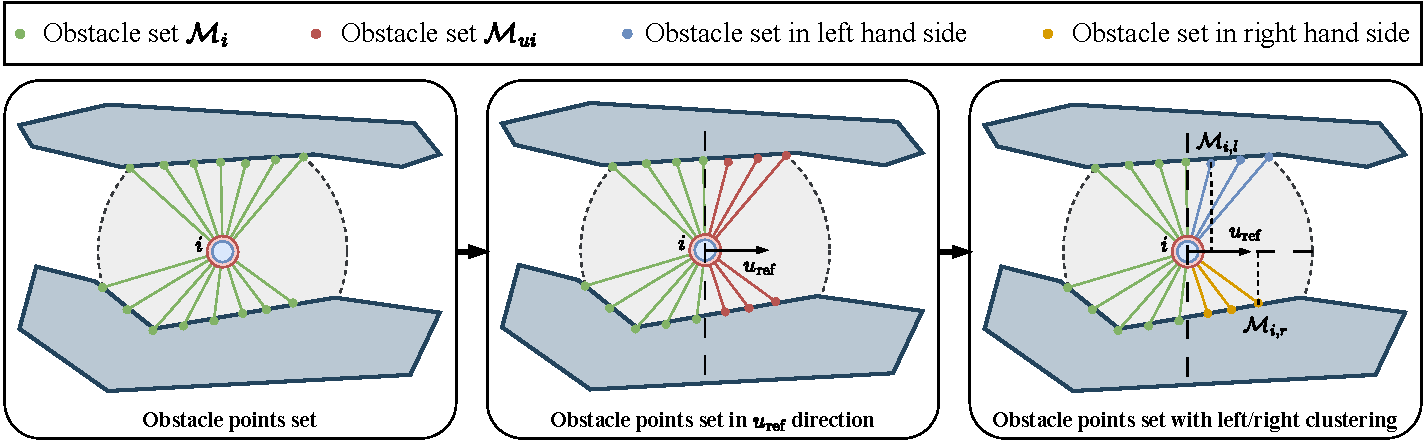
\includegraphics[width=\textwidth]{paper3/images/perception.pdf}
    \caption{The process of estimating the environment's width: the robot first obtains point cloud data $\mathcal{M}_i$ from the local sensor (green). It then selects a point set $\mathcal{M}_{ui}$ (red) that is in front of the robot in a predefined direction $u_\text{ref}$. It then divides those points into two sub-sets on the left-hand (blue) and right-hand (yellow) sides. Finally, the points that are nearest to the robot in $u_\text{ref}$ direction in each side, $\mathcal{M}_{i,l}$, and $\mathcal{M}_{i,r}$ are selected to estimate the width of the environment.}
    \label{fig:perception}
\end{figure*}

In this section, details about making the state-changing decision and computing the scaling factor $\kappa$ of the desired formation are presented. To estimate the environment's width, each robot $i$ only considers the obstacle point set, $\mathcal{M}_{ui}$, in the $u_\text{ref}$ direction. It is given by
\begin{equation}
    \mathcal{M}_{ui} = \left\{\mathcal{M}_{i}\vert\left\langle\left(p_i-\mathcal{M}_{i}\right),u_\text{ref}\right\rangle<0\right\}
    \label{eqn:mui}
\end{equation}

By using the DBSCAN~\cite{10.5555/3001460.3001507} technique, the obstacle point set $\mathcal{M}_{ui}$ is clustered into two clusters on the left and right sides of the robot in $u_\text{ref}$ direction. Denote $\mathcal{M}_{i,l}$ and $\mathcal{M}_{i,r}$ respectively as the obstacle point on the left and right sides whose distance to the robot $i$ is minimum. The width of the environment can be estimated as follows:
\begin{equation}
    w_e= \left\vert\left\langle\left(\mathcal{M}_{i,r}-\mathcal{M}_{i,l}\right),u_\text{ref}\right\rangle\right\vert
    \label{eqn:we}
\end{equation}

The estimation of the environment's width can be depicted in Fig.~\ref{fig:perception} and described in Alg.~\ref{alg:we}. Besides, the formation's width $w_f$ can be easily determined through the predefined formation topology. Given the widths of the environment and formation, the scaling factor $\kappa$ can be computed as follows:
\begin{equation}
    \kappa=\dfrac{w_e-2r}{w_f}
    \label{eqn:kappa}
\end{equation}


\begin{algorithm}
\caption{Pseudocode to estimate the environment's width}
\label{alg:we}
Get obstacle point set $\mathcal{M}_{ui}$ in front of robot $i$ in motion direction $u_\text{ref}$\tcc*[r]{Eq. \ref{eqn:mui}}
Cluster obstacle point set $\mathcal{M}_{ui}$ to left and right hands of robot using DBSCAN\;
Find the pair of obstacle points $\left(\mathcal{M}_{i,l},\mathcal{M}_{i,r}\right)$, whose distance to $u_\text{ref}$ is minimum\;
Obtain the environment's width $w_e$\tcc*[r]{Eq. \ref{eqn:we}}
\Return $w_e$\;
\end{algorithm}

\begin{algorithm}[h!]
\caption{Pseudocode of the MPPDC strategy}
\label{alg:our}
Get the observed obstacle points $\mathcal{M}_i$\;
\If{$\mathcal{M}_i$ is empty}{
    mode $\leftarrow$ \textit{``Formation''}\;
    $\kappa \leftarrow 1.0$\;
}
\Else{
    Get the environment's width $w_e$\tcc*[r]{Alg. \ref{alg:we}}
    \If{$w_e$ is None}{
        mode $\leftarrow$ \textit{``Formation''}\;
        $\kappa \leftarrow 1.0$\;
    }
    \Else{
        \If{$w_e\leq\lambda r$}{
            mode $\leftarrow$ \textit{``Tailgating''}\;
        }
        \Else{
            mode $\leftarrow$ \textit{``Formation''}\;
            Estimate the desired formation width $w_f$\;
            \If{$w_e-2r\leq w_f$}{
                Compute the scaling factor $\kappa$\tcc*[r]{Eq. \ref{eqn:kappa}}
            }
            \Else{
                $\kappa\leftarrow1.0$\;
            }
        }
    }
}
\Switch{mode}{
\Case{``Formation''}
{
    Get the desired trajectory $p_i^*$\tcc*[r]{Eq. \ref{eqn:formation}}
}
\Case{``Tailgating''}
{
    Select leader to follow\tcc*[r]{Alg. \ref{alg:ls}}
    Get the desired trajectory $p_i^*$\tcc*[r]{Eq. \ref{eqn:tailgating}}
}
}
Formulate the cost function and solve the MPC problem to obtain the optimal control signal $u_i^*$\tcc*[r]{Eqs. \ref{eqn:J}-\ref{eqn:constraints}}
\Return $u_i^*$\;
\end{algorithm}

As a result, each robot $i$ can choose its mode and compute scaling factor $\kappa$. It then computes the desired trajectory corresponding to its mode and the optimal control signal using MPC, as presented in Alg.~\ref{alg:our}. This problem can be solved be commonly used, nonlinear programming (NLP)
solvers, such as the Sequential Least Squares Programming (SLSQP)~\cite{kraft1988software}. We implemented the MPC model in Python with the help of a state-of-the-art optimization software library~\cite{2020SciPy-NMeth} to find the solution to the problem.